\section{Stochastic Edge Acceptance}
After reading a lot about other models for evolving graphs I decided to come up with a new model for adding edges with an added element of randomness.
The working name for the model is Stochastic Edge Acceptance or SEA for short.
In most models the edges selected for evaluation are random but which edge is actually chosen to be added to the graph is deterministic.
Random processes occur all the time in the natural world around us, therefore, I believe that this added element of randomness helps better represent a natural system.
One might wonder what sort of system this could represent, so let us consider a network where a node considers joining a cluster and usually prefers to join the smaller cluster but there is still a probability that it instead chooses to join the larger cluster.

The underlying idea is to have a process which favors the minimization of the largest cluster through considering multiple edges at each step in the evolution algorithm, therefore, it is an Achlioptas process.
This is a local rule, i.e. it only considers local information such as the size of the clusters to which the nodes in the considered edge belong.
I wanted to create a simple probability using only the sizes of the clusters corresponding to the considered edges.
Also note in the algorithm below that intra-cluster edges are always accepted.

A form of the algorithm can be written in pseudocode as follows:
\begin{itemize}
	\item Let $T$ be the total number of edges to add to the graph.
	\item Let $A_t = \{e_1, e_2, ..., e_t\}$ be the set of accepted edges at step $t$.
	\item Let $e_t^1$ and $e_t^2$ be the two nodes which edge $e_t$ would connect.
	\item Let $C(e_t^i)$ be the cluster which $e_t^i$ belongs to.
	\item Let $C(e_t)$ be the cluster which would be formed by activating $e_t$.
	\item Let $r \in [0, 1)$ be a randomly generated number.
	\item Let $p = \frac{C(e_t)^{-1}}{C(e_t)^{-1} + C(e_t')^{-1}}$
\end{itemize}

\begin{algorithm}
	\caption{Stochastic Edge Acceptance}\label{Stochastic-Edge-Acceptance}
	\begin{algorithmic}[1]
		\Procedure{SEA}{$T$}
		\State $A \gets \emptyset$
		\State $t \gets 1$

		\While{$t \le T$}
			\If{$C(e_t^1) = C(e_t^2)$}
				\State $A \gets A \cup \{e_t\}$
				\State $t \gets t+1$
			\ElsIf{$C(e_t'^1) = C(e_t'^2)$}
				\State $A \gets A \cup \{e_t'\}$
				\State $t \gets t+1$
			\ElsIf{$p$ < r}
				\State $A \gets A \cup \{e_t\}$
				\State $t \gets t+1$
			\Else
				\State $A \gets A \cup \{e_t'\}$
				\State $t \gets t+1$
			\EndIf
		\EndWhile
	\EndProcedure
	\end{algorithmic}
\end{algorithm}

Fig. \ref{fig:ER_BF_PR_SEA_transition} below illustrates the SEA model in comparison with ER, BF, and PR models.

\begin{figure}[H]
	\centering
	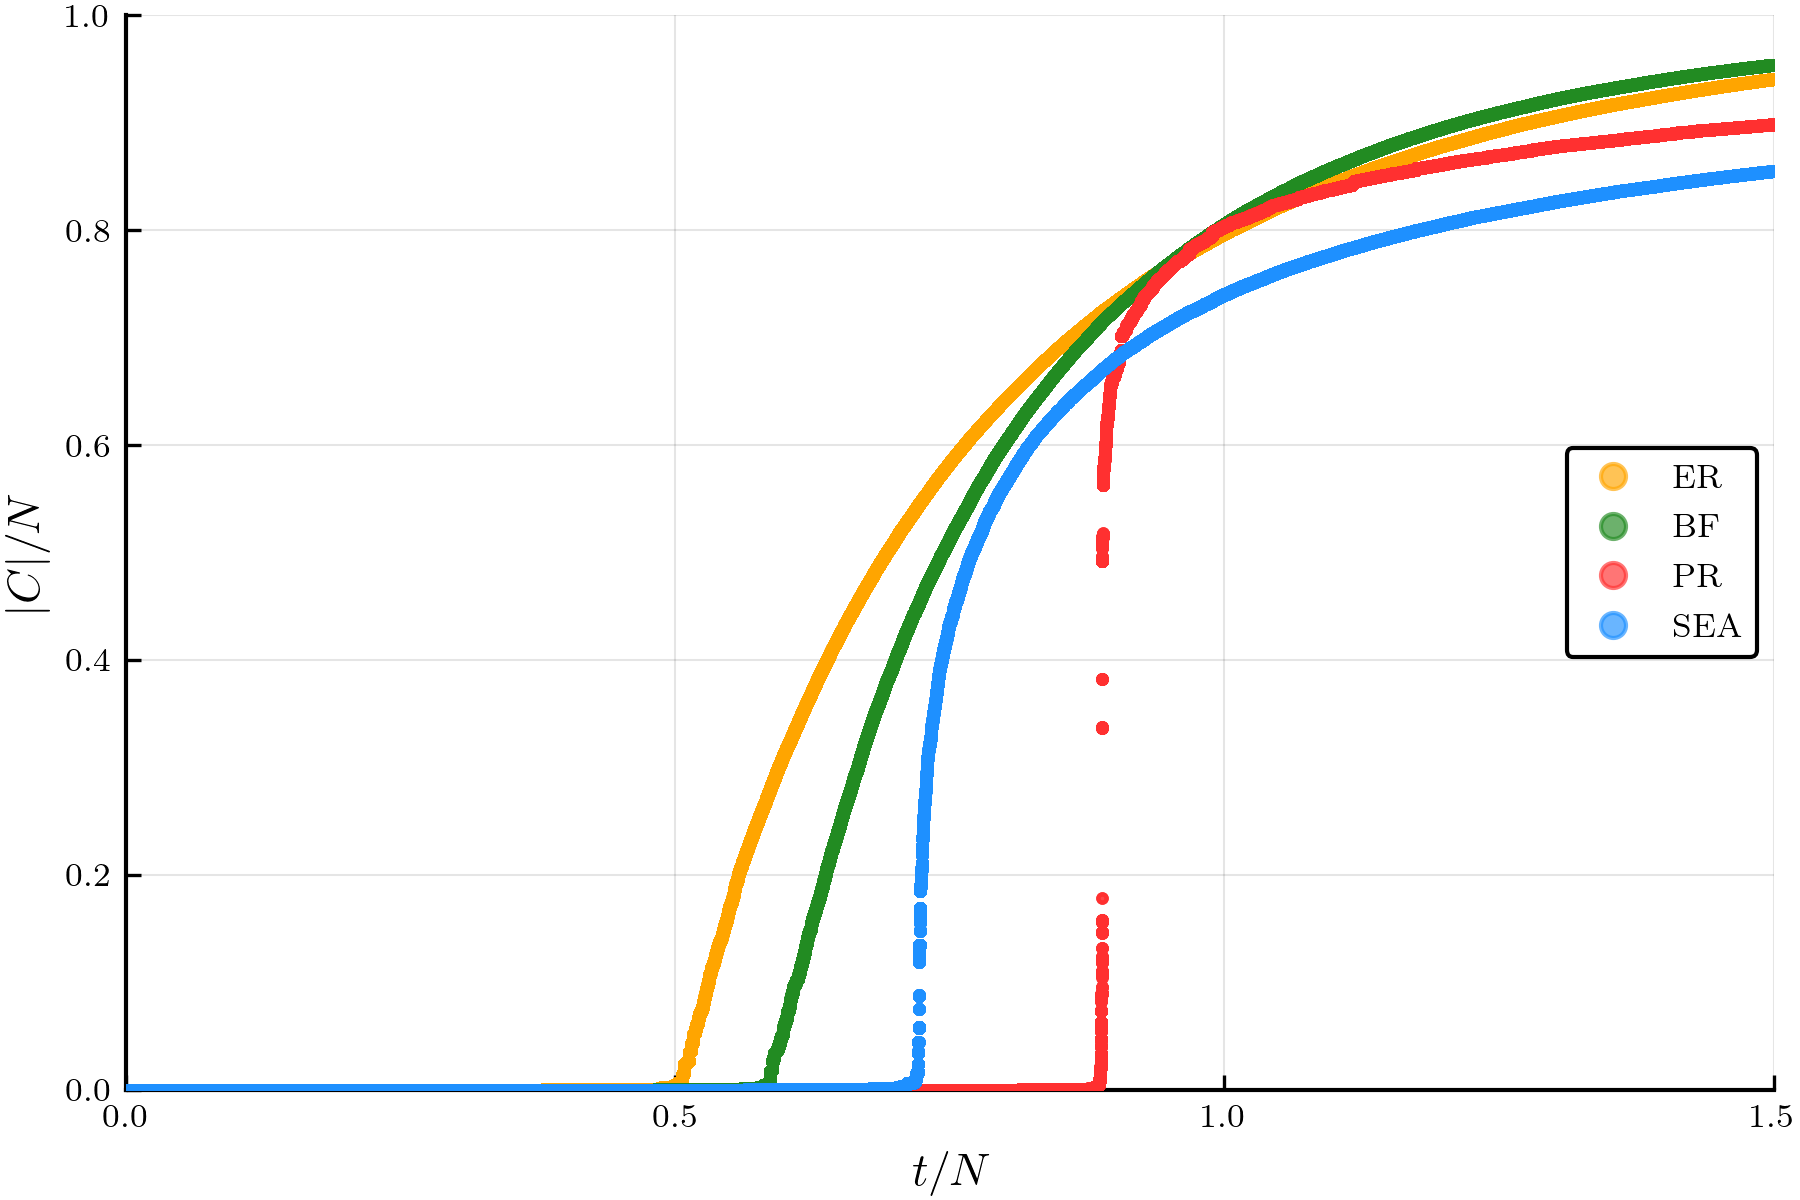
\includegraphics[width=350pt, clip]{images/Network_ER_BF_PR_SEA_1e6_order_param.png}
	\caption{Stochastic Edge Acceptance Model Order Parameter, $N = 10^6$}
	\label{fig:ER_BF_PR_SEA_transition}
\end{figure}

Fig. \ref{fig:delta_scaling_2} (uses data from an ensemble average of 1000 simulations) shows two curves corresponding to steps in the evolution process.
$r = t_0$ represents the point where the cluster heterogeneity peaks and $r = t_1$ represents the point where the order parameter jumps by the largest amount.
The data tells us that the system undergoes a phase transition around $r = 0.718655 \pm 0.002862848$.

\begin{figure}[H]
	\centering
	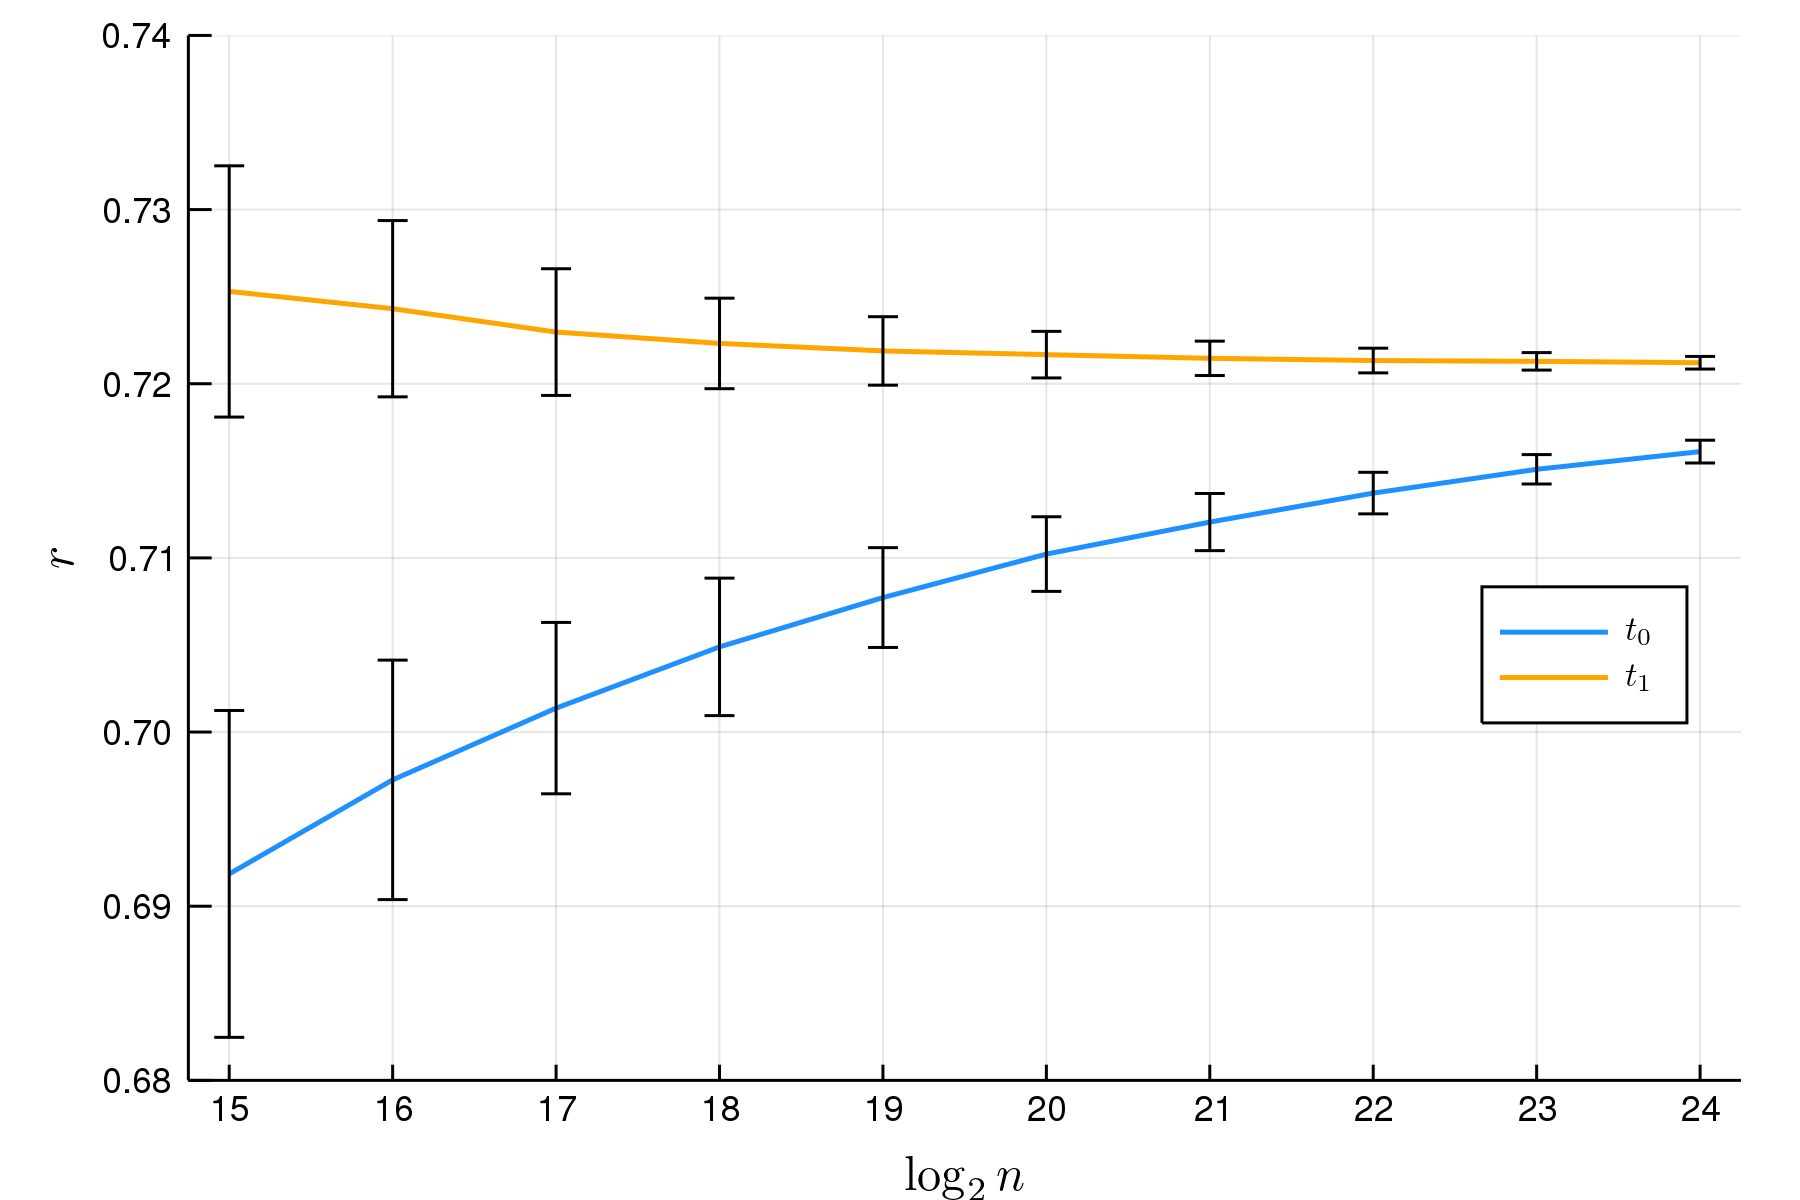
\includegraphics[width=350pt, clip]{images/delta_scaling_2.png}
	\caption{Stochastic Edge Acceptance Phase Transition Point Identification, $N = 10^6$}
	\label{fig:delta_scaling_2}
\end{figure}

Fig. \ref{fig:Network_stochastic_edge_acceptance_observables} shows how the observables scale as a function of the system size $N = 2^k, k \in \{15, 16, ..., 23, 24\}$.

\begin{figure}[H]
	\centering
	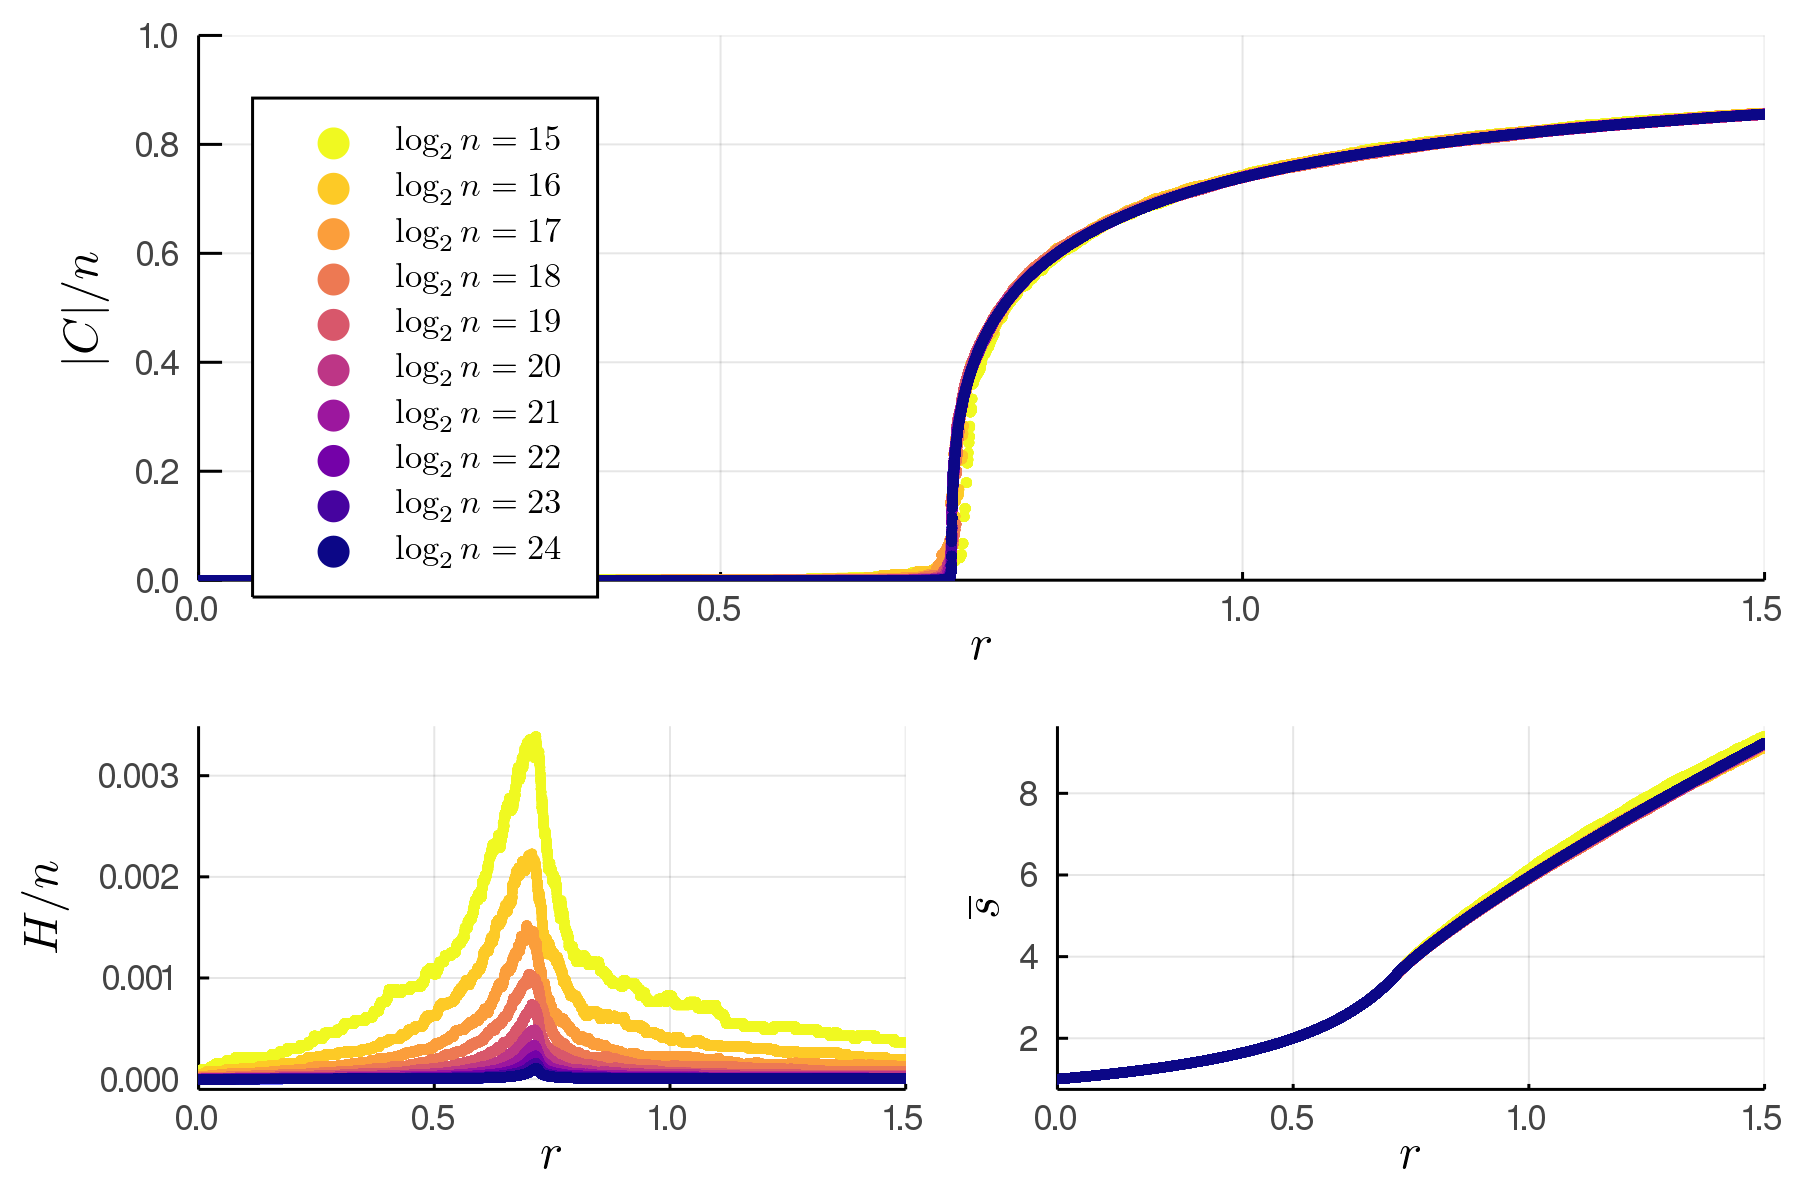
\includegraphics[width=350pt, clip]{images/Network_stochastic_edge_acceptance_observables.png}
	\caption{Stochastic Edge Acceptance Model, $N = 10^6$}
	\label{fig:Network_stochastic_edge_acceptance_observables}
\end{figure}

Now one might wonder how do these models look when applied to a lattice.
The way the simulation library was designed makes it easy to run the same simulations on a different lattice, so we're in luck.

Fig. \ref{fig:Lattice2D_ER_BF_PR_SEA_transition} illustrates what happens when we change the graph type to a 2D square lattice allowing only edges between nearest neighbors.
Changing the graph to be a 2D lattice we see the order parameter shifts to a later point, which makes sense due to the fact that in a two dimensional lattice each point only has four neighbors thus only four possible edges it can be connected with.

\begin{figure}[H]
	\centering
	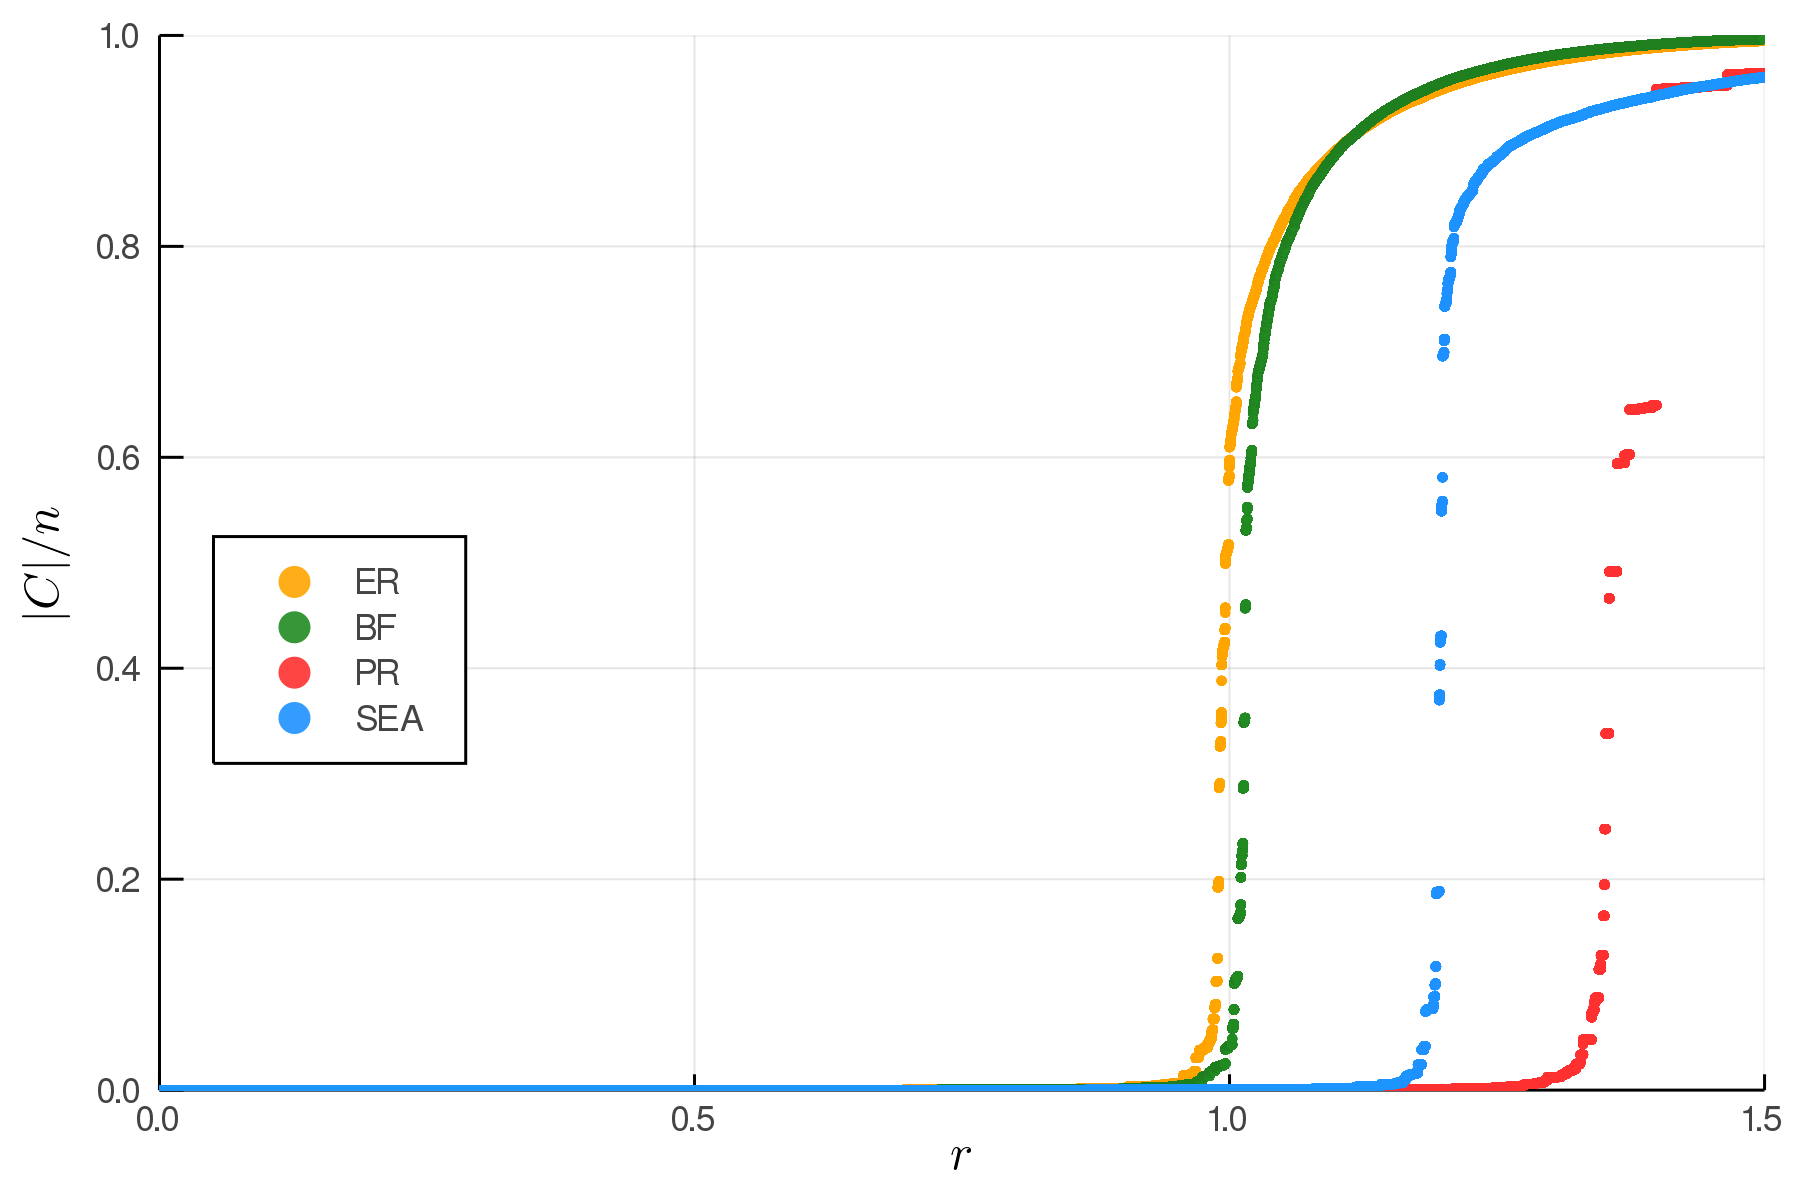
\includegraphics[width=350pt, clip]{images/Lattice2D_ER_BF_PR_SEA_1e6_order_param.png}
	\caption{Stochastic Edge Acceptance Model Order Parameter on a 2D Lattice, $L = 10^3$}
	\label{fig:Lattice2D_ER_BF_PR_SEA_transition}
\end{figure}

Fig. \ref{fig:Lattice3D_ER_BF_PR_SEA_transition} illustrates the case of allowing only nearest neighbor edges on a 3D cubic lattice.

\begin{figure}[H]
	\centering
	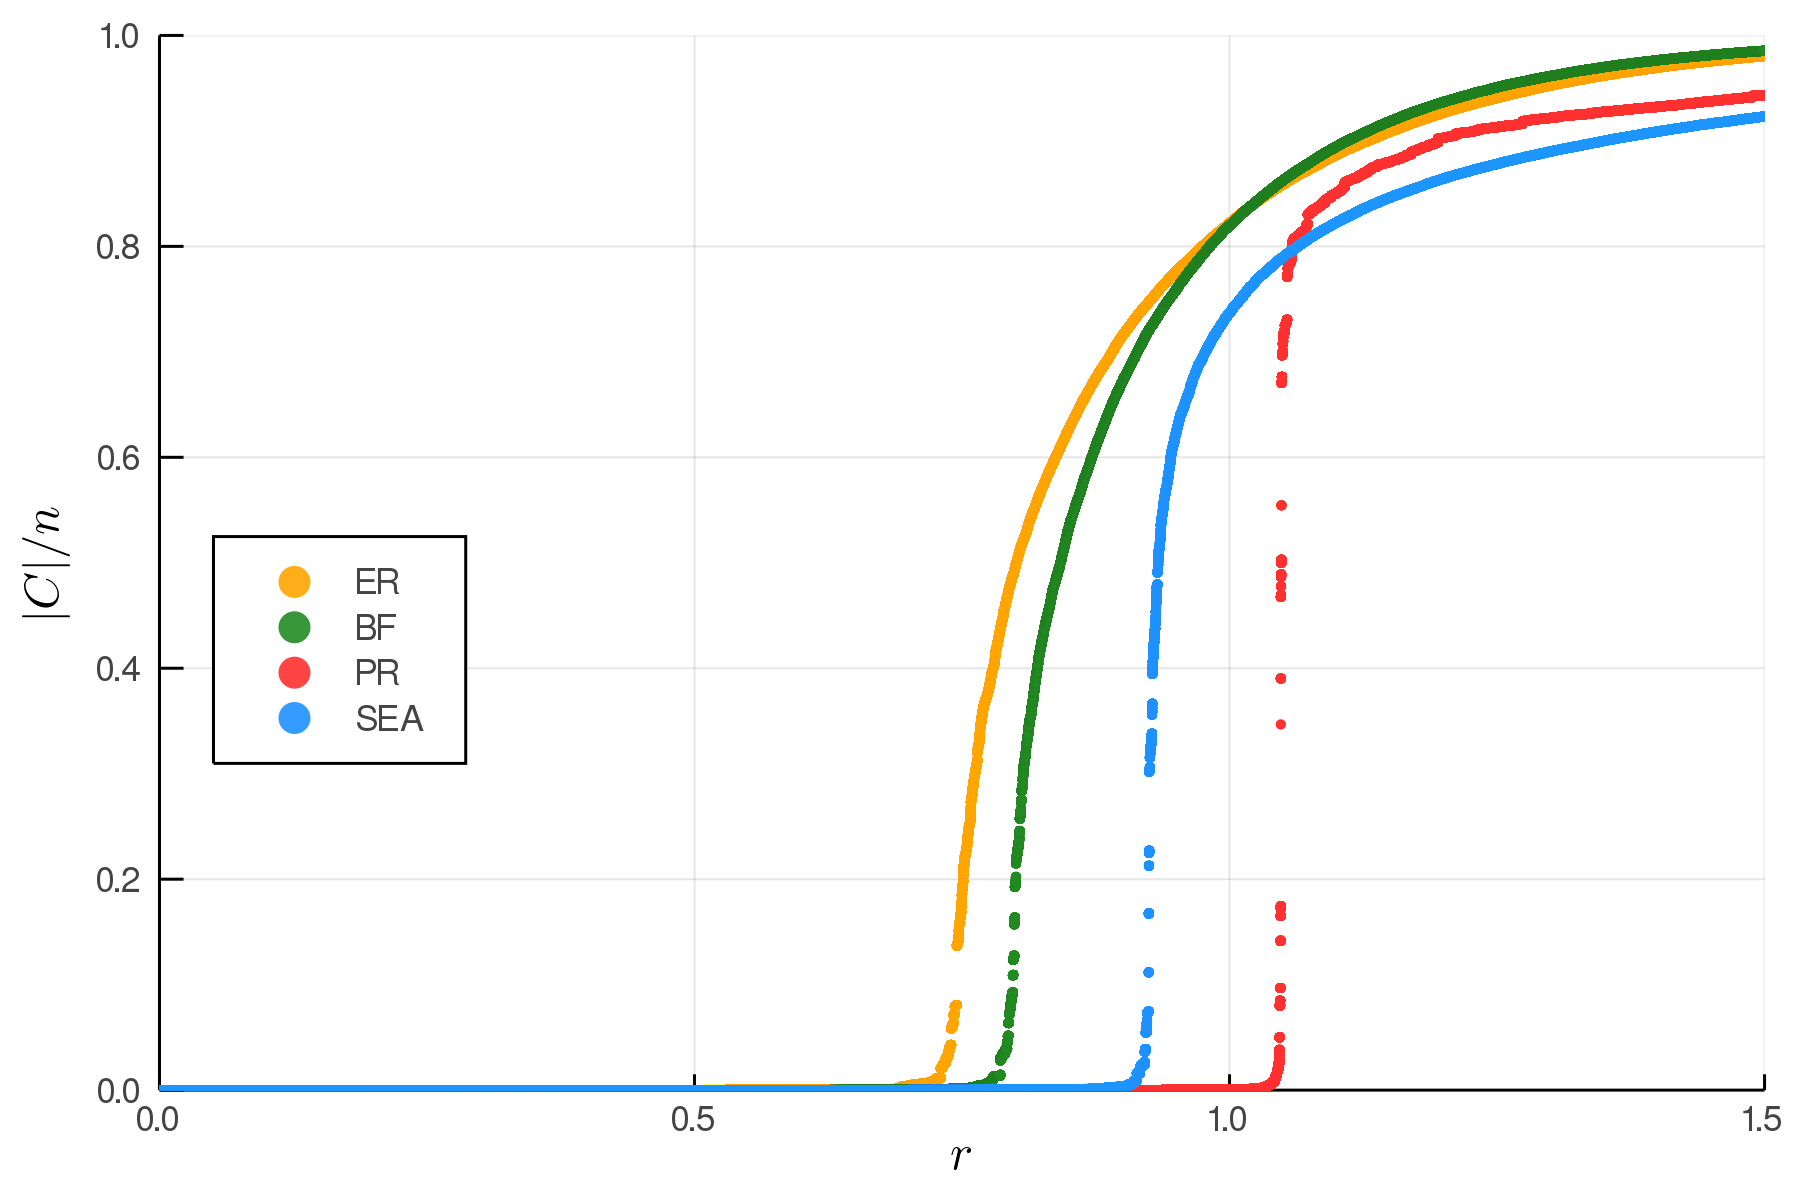
\includegraphics[width=350pt, clip]{images/Lattice3D_ER_BF_PR_SEA_1e6_order_param.png}
	\caption{Stochastic Edge Acceptance Model Order Parameter on a 3D Lattice, $L = 10^2$}
	\label{fig:Lattice3D_ER_BF_PR_SEA_transition}
\end{figure}
